\documentclass[11pt]{article}
% \documentclass[twocolumn]{article}

\usepackage[francais]{babel}
\usepackage[utf8]{inputenc}
\usepackage{enumerate}
\usepackage{amssymb}
\usepackage{amsfonts}
\usepackage{amsthm}
\usepackage{graphicx}
\usepackage[ruled,vlined,french]{algorithm2e}

% New commands
\newcommand{\xt}{$(X_t)$ }
\newcommand{\om}{$\Omega$ }
\renewcommand\qedsymbol{$\blacksquare$}


% \renewcommand\diffsim{$x \bigtriangleup y$}

% New Environment
\newtheorem{theorem}{Théorème}
\newtheorem{conjecture}{Conjecture}
\newtheorem{propriete}{Propriété}[subsection]
\newtheorem{proposition}{Proposition}[subsection]
\newtheorem{corollary}{Corollaire}[subsection]
\newtheorem{definition}{Définition}[subsection]
\newtheorem{lemme}{Lemme}[subsection]
\newtheorem{remarque}{Remarque}[subsection]




\begin{document}

\title{Génération aléatoire de polytopes en nombres entiers en utilisant les chaînes de Markov}
\author{Julien David, Lionel Pournin, Rakotonarivo Rado}
\maketitle

\noindent{\textbf{Résumé.}} Ce document va décrire une approche pour faire de la génération aléatoire de polytope entiers en utilisant les chaînes de Markov, de la construction du générateur à l'optimisation de celui-ci. Les objets à engendrer sont les polytopes entiers contenus dans l'hypercube ${[0,k]}^d$, notés $(d,k)$-polytopes. La construction du générateur aléatoire se fait de la manière suivante~: modéliser une chaîne de Markov dont les états seront les $(d,k)$-polytopes, lancer des marches sur la chaîne jusqu'à ce qu'on atteigne une distribution stationnaire. On va montrer que cette distribution stationnaire est unique et uniforme. De ce fait, on aura construit un générateur aléatoire uniforme de $(d,k)$-polytopes.

% Eventuellement ajouter plus tard les résultats

\vspace*{12pt}

\section{Introduction}

Une chaîne de Markov est un processus qui évolue en temps sur un ensemble d'états \om et est caractérisée par sa matrice de transition $P$, qui décrit les transitions entre les états de $\Omega$.

L'idée principale de la génération aléatoire en utilisant les chaînes de Markov est la suivante~: modéliser une chaîne de Markov dont les états seront les objets à engendrer, lancer des marches sur la chaîne jusqu'à ce qu'on atteigne une distribution stationnaire. L'uniformité du générateur sera conditionnée par la distribution stationnaire de la chaîne de Markov ainsi modélisée. Cette approche va être utilisée pour notre cas dans la génération de polytopes en nombres entiers contenus dans l'hypercube ${[0,k]}^d$, notés $(d,k)$-polytopes.

Bien que l'idée de laquelle on part soit simple, il y a cependant plusieurs difficultés dans le cas des $(d,k)$-polytopes~: nous n'avons pas d'information exacte sur la taille de notre espace des états, la matrice de transition n'est pas entièrement déterminée, et enfin, assurer une distribution uniforme nécessite que certaines conditions sur cette dérnière soient vérifiées.

Toutefois, se baser sur une chaîne de Markov semble être une piste sérieuse vu les nombreux résultats et différentes techniques qui sont déjà à notre disposition \cite{levin2009markov}. Il y a également le fait qu'on peut faire des essais expérimentaux: modéliser notre chaîne et lancer une batterie de tests dessus.

Le travail sur cette approche sera principalement de:
\begin{itemize}
  \item Trouver des opérations locales sur nos $(d,k)$-polytopes pour pouvoir passer d'un état à un autre.
  \item Utiliser les techniques et les résultats connus sur les chaînes de Markov pour estimer le temps de mélange.
  \item Réfléchir sur des idées de preuves pour l'uniformité du générateur.
\end{itemize}

Ce document sera structuré de la manière suivante. Dans un premier temps, un bref rappel des principaux résultats sur les chaînes de Markov - tous essentiellement proviennent de notre lecture de \cite{levin2009markov}. Et dans un deuxième temps notre modèle concret de générateur en utilisant les chaînes de Markov.

\section{Chaînes de Markov}

Le nombre de polytopes entiers dans ${[0,k]}^d$ est finis, par conséquent on va s'interesser aux chaînes de Markov à espace d'états fini. Dans toute la suite du document, on supposera que la chaîne de Markov étudiée est une chaîne à espace d'états fini.

\subsection{Définitions}

Une chaîne de Markov à espace d'états fini $(X_t)_{t\geq{0}}$ est un processus qui évolue en temps sur les éléments d'un espace $\Omega$ fini. Le déplacement d'un état $x \in \Omega$ à un autre état de $\Omega$ suit une distribution fixe $P(x,\cdot)$. C'est une séquence de variables aléatoires $(X_0, X_1, \cdots)$ à valeur dans $\Omega$.

La valeur de \xt étant l'état de la chaîne à l'instant $t$, la \textbf{propriété de Markov} sur \xt assure que l'état à l'instant $t+1$ ne dépend que de l'état à l'instant $t$.

La matrice de transition $P$ de \xt qui décrit les transitions entre les états de \om est une matrice stochastique dont la $x-$ème ligne désigne la distribution $P(x,\cdot)$. On a:

\begin{equation}
  \sum_{y \in \Omega} P(x,y) = 1 \quad \forall{x \in \Omega}
\end{equation}

\begin{figure}
  \begin{center}
    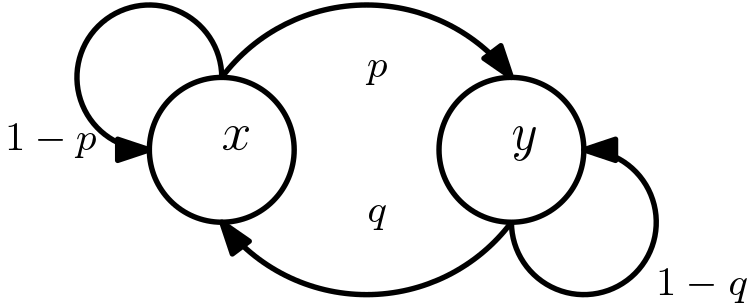
\includegraphics[width=5cm]{assets/frog}
    \caption{Une chaîne de Markov telle que: $\Omega = \{x,y\}$, $P(x,x) = 1-p$, $P(x,y) = p$,  $P(y,x) = q$ et $P(y,y) = 1-q$}
    \label{fig:fig1}
  \end{center}
\end{figure}

\subsection{Propriétés}

Soient $(X_t)_{t\geq{0}}$ une chaîne de Markov, \om son espace des états et $P$ sa matrice de transition.

\subsubsection{Irréductibilité}

La matrice P de $X_t$ est \textbf{irréductible} si tout état $x$ de \om est accessible depuis n'importe quel état de $\Omega$. En d'autres mots, cela signifie que le graphe de $X_t$, dont les sommets sont les états de $\Omega$ et les arêtes les relations de transitions entre les états de $\Omega$, est fortement connexe. Formellement, on a:

\begin{equation}
  \exists r_0 \quad \ : \quad \forall r > r_0, \  \forall x,y \in \Omega \quad P^r(x,y) > 0
\end{equation}

\subsubsection{Périodicité}

On définit par $\mathcal{T}(x):=\{t\geq{1} \ : P^t(x,x)>0\}$, l'ensemble des temps où la chaîne retourne en $x$. La \textbf{période} de $x$ est définit par $\mathrm{pgcd}(\mathcal{T}(x))$.

\begin{propriete} \label{prop1}
  Si $P$ est irreductible alors tous les états de \om ont la même période.
\end{propriete}

$X_t$ est dite \textbf{apériodique} si tous les états de \om ont pour période 1, sinon elle est dite \textbf{périodique}.

\subsubsection{Symétrie}

On dit que $X_t$ est \textbf{symétrique} si pour tout $x$ et $y$ de \om, la probabilité de passer de $x$ en $y$ et la probabilité de passer de $y$ en $x$ sont égales; i.e.:

\begin{equation}
  P(x,y) = P(y,x) \quad \forall x,y \in \Omega
\end{equation}


\subsubsection{Hitting time et premier temps de retour}

Pour tout état $x \in \Omega$ on défini le \textbf{hitting time} par:

\begin{equation}
  \tau_x:=\min \{t\geq{0} \ : X_t = x\},
\end{equation}

le premier moment où la chaîne visite $x$. en particulier, le \textbf{premier temps de retour} en $x$ est définit par:

\begin{equation}
  \tau_x^+:=\min \{t\geq{1} \ : X_t = x\} \quad \mathrm{si} \quad X_0 = x
\end{equation}

\subsection{Récurrence d'un état}\label{recurrence}

Un état $x$ est dit \textbf{récurrent positif} si $\mathrm{E}_x(\tau_x^+)<\infty$, où $\mathrm{E}_x(\tau_x^+)$ est l'espérence du premier temps de retour en $x$ en partant de $x$. Cette quantité représente l'intervale de temps typique entre deux passages consécutifs en $x$.

\subsection{Distribution stationnaire}

On note par $\mu_t$ le vecteur ligne qui donne la distribution de probabilité sur \om à l'instant $t$ et par $\mu_t(x)$ la probabilité d'être en $x$ à l'instant $t$, i.e. $\mu_t(x) = \mathbf{P}\{X_t = x \} \quad \forall x \in \Omega$. Obtenir la distribution à l'instant $t+1$ revient à appliquer une fois à $\mu_t$ la matrice de transition $P$ par la droite. On a:

\begin{equation}
  \mu_t = \mu_{t-1}P \quad \forall t\geq{1}
\end{equation}

En partant d'une distribution initiale $\mu_0$, on a:

\begin{equation}
  \mu_t = \mu_0P^t \quad \forall t\geq{0}
\end{equation}

Une distribution $\pi$ est dite \textbf{stationnaire} pour \xt si elle satisfait

\begin{equation}
  \pi = \pi P
\end{equation}

De manière équivalente:

\begin{equation}
  \pi(y) = \sum_{x \in \Omega} \pi(x)P(x,y) \quad \forall y \in \Omega
\end{equation}

La distribution stationnaire peut être perçue comme étant la représentation du temps passé en chaque état $x$ de $\Omega$.

\subsection{Temps de mélange}

Le \textbf{temps de mélange} est le temps minimum pour atteindre la distribution stationnaire si elle existe. Dans notre cas, comme on veut atteindre une distribution uniforme, le temps de mélange nous donne une idée sur l'éfficacité de notre générateur.

Plusieurs résultats de \cite{levin2009markov} nous donnent des bornes (inférieures et supérieures) sur le temps de mélange. Ces résultats seront rappelés et utilisés plus tard dans nos preuves.

\subsection{Existence et unicité de $\pi$}

L'existence de la distribution stationnaire pour une chaîne irreductible est fortement liée à $\tau_x^+$, en particulier à la recurrence de $x$ (\ref{recurrence}). Pour une chaîne \xt irreductible et apériodique ont a les propriétés suivantes:

\begin{propriete}\label{prop:prop22}
  Si P est irreductible et apériodique, les deux assertions suivantes sont équivalentes:
  \begin{enumerate}[i]
    \item Il existe $\pi$, une distribution sur \om tel que $\pi = \pi P$ et $\pi(x)>0$ pour tout $x$ de \om.
    \item $\pi(x) = \frac{1}{\mathrm{E}_x(\tau_x^+)}$
  \end{enumerate}
\end{propriete}

\begin{propriete}\label{prop:prop23}
  Une chaîne irreductible à espace d'états fini est récurrente positive, i.e. tous ces états sont récurrents positifs. Elle possede une unique distribution stationnaire $\pi$.
\end{propriete}

\begin{propriete}\label{prop:prop24}
  Si \xt est symétrique alors la distribution uniforme sur \om est stationnaire.
\end{propriete}

\section{Modèle des $(d, k)$-polytopes}

Rappelons que notre objectif principal est de construire un générateur aléatoire uniforme de $(d, k)$-polytopes. Et cela en utilisant les chaînes de Markov. Considérons notre hypercube $[0,k]^d$. L'idée générale de la construction du générateur aléatoire est de lancer des marches sur une chaîne de Markov \xt dont l'espace des états \om est l'ensemble des $(d, k)$-polytopes pour $k$ et $d$ fixés et la matrice de transition $P$, n'étant pas entièrement déterminée, est définie par des opérations locales sur nos $(d, k)$-polytopes.

Nous allons prouver que \xt ainsi définie aura l'uniforme comme distribution stationnaire et ainsi obtenir un générateur uniforme de $(d, k)$-polytopes.

\subsection{Notations et contexte du générateur}

Il est utile de préciser les quelques notations que l'on va utiliser dans toute la suite du document.

% $$
% \Omega := \{x : x \  est \  une \  enveloppe \  convexe \  de \  l \  points\}
% $$

L'espace des états \om de \xt est l'ensemble des $(d,k)$-polytopes. Un état $x$ de \om est un ensemble de $l$ points qui constituent exactement une enveloppe convexe à $l$ sommets, i.e. $x=\{v_1, v_2, …, v_l\}$ avec $v_i\in[0,k]^d$ pour tout $i \in [1,l]$. On observe alors que $Conv(x) = x$. Dans certains contextes on préfèrera faire référence à l'enveloppe convexe $Conv(\cdot)$ quand des opérations locales seront appliquées à nos états.

On notera par $|x|$ le nombre de sommets de $x$.

Soit $x=\{v_1, v_2, …, v_l\} \in \Omega$. On considère:
\begin{enumerate}
  \item $x-\{v_j\}$ l'enveloppe convexe auquel on a retiré exactement le $j$-ème sommet de $x$. On remarque que $x-\{v_j\}$ n'est de dimension pleine que si $|x|>d+1$.
  \item $x \cup \{v\}$, où $v \in [0,k]^d$, l'enveloppe convexe auquel on a ajouté exactement un point à $x$ sans avoir retiré aucun des $l$ sommets de $x$. On observe que $|x \cup \{v\}| = |x| + 1$.
\end{enumerate}


\subsection{Règles de transition}\label{sec:regles}

Les règles de transition sur notre espace \om est définie par des opérations locales sur nos $(d, k)$-polytopes, des opérations qui consistent à ajouter ou supprimer un sommet pour passer d'un état à un autre.

Soient $x$ et $y$ deux états de $\Omega$. On tire uniformément un point $v$ dans $[0,k]^d$. On se donne les règles suivantes:
\begin{itemize}
  \item Si $v$ est un point intérieur à $x$; $v$ appartient à l’enveloppe convexe de $x$ mais n’est pas dans $x$, on boucle sur $x$
  \item Si $v$ appartient à $x$:
  \begin{itemize}
    \item Si $x$ a au moins $d+2$ sommets alors on supprime $v$ de $x$. On a une transition de $x$ vers $y = x - \{v\}$
    \item Sinon si $x$ est un simplexe:
      \begin{itemize}
        \item On choisit de déplacer $v$
        \item Sinon on boucle sur $x$
      \end{itemize}
  \end{itemize}
  \item Si $v$ est tiré à l'extérieur de l'enveloppe convexe de $x$, on calcule l'enveloppe convexe de $x \cup \{v\}$:
  \begin{itemize}
    \item Si l’ensemble des sommets de l’enveloppe convexe de $x\cup\{v\}$ est exactement $x\cup\{v\}$, alors on a une transition de $x$ vers $y = x \cup \{v\}$
    \item Sinon on boucle sur $x$
  \end{itemize}
\end{itemize}

\begin{figure}
  \begin{center}
    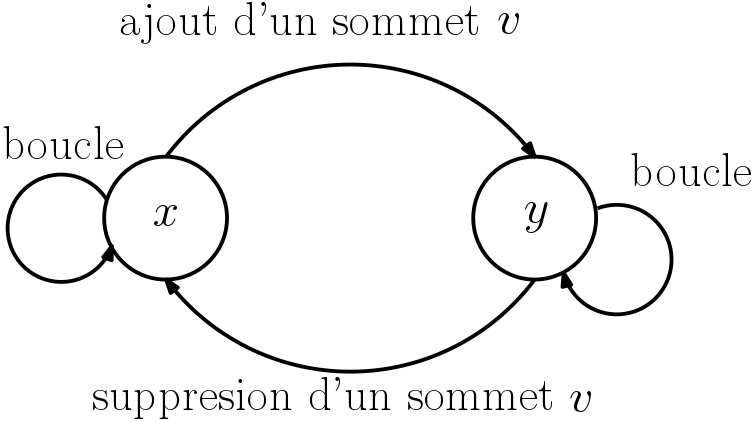
\includegraphics[scale=0.3]{assets/transition}
    \caption{Relation de transition entre deux états $x$ et $y$ de \om: $y = x \cup \{v\}$ et $x = y - \{v\}$, où $v \in [0,k]^d$.}
    \label{fig:fig2}
  \end{center}
\end{figure}

\begin{figure}
  \begin{center}
    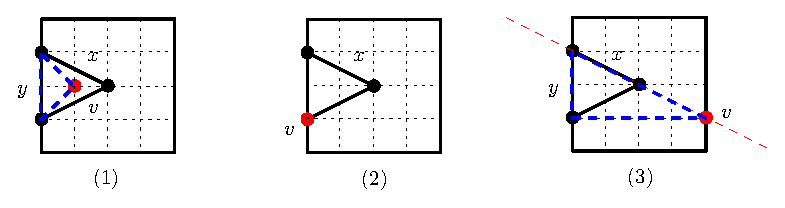
\includegraphics[scale=0.9]{assets/boucle}
    \caption{Pour $[0,4]^2$. Exemples de cas où on a une boucle sur $x$: (1) $v$ est un point intérieur à $x$, $P(x,y) = 0$. (2) $v \in x$ et $|x| < d+2$. (3) $v$ est tiré à l'extérieur de $Conv(x)$ et $|Conv(x\cup\{v\})| \neq |x|+1$, $P(x,y) = 0$. }
    \label{fig:boucle}
  \end{center}
\end{figure}

\subsection{Marches sur \xt}

Considérons maitenant notre chaîne \xt ainsi définie. Engendrer aléatoirement un $(d, k)$-polytope consiste à effectuer une marche aléatoire sur \om avec les règles de transition que l'on a précédement définies jusqu'à ce qu'on atteigne la distribution stationnaire.

Et justement ce temps d'arrêt de notre marche, qui est exactement le temps de mélange de $X_t$, sera déterminé par des conditions qu'il nous faut encore établir de manière à optimiser l'efficacité de notre générateur. Plusieurs techniques sont à notre disposition mais elles seront étudiées plus tard.

Engendrer aléatoirement un $(d, k)$-polytope, en se basant sur ce modèle de chaîne de Markov est donné par l'algorithme suivant:

\vspace{0.5cm}

\begin{algorithm}[H]\label{Algo.RS}
  \LinesNumbered
  \DontPrintSemicolon
  \KwIn{the dimension $d$, the size $k$ of the hypercube}
  \KwOut{a random lattice $(d,k)$-polytope}
  \BlankLine

  sample a random lattice $(d,k)$-simplex $P$ with vertex set $\mathcal{V}$\;
  \While{we are not close enough to the stationary distribution}{
  generate a random lattice point $x$ in $[0,k]^d$\;
  \If{$x \in \mathcal{V}$ and $\mathrm{conv}(\mathcal{V}\mathord{\setminus}\{x\})$ is $d$-dimensional}{
    $P \leftarrow \mathrm{conv}(\mathcal{V}\mathord{\setminus}\{x\})$\;
   }
  %\Else{$|\mathrm{conv}(\mathcal{V} \cup \{x\})|$ == $|\mathcal{V}| + 1$}{
  \Else{
    compute the convex hull $Q$ of $\mathcal{V}\cup\{x\}$\;
    \If{the vertex set of $Q$ is $\mathcal{V}\cup\{x\}$}{
      $P \leftarrow \mathrm{conv}(\mathcal{V} \cup \{ x\})$\;
    }
  }
 }
 \Return{$P$}
 \caption{Random sampling of a lattice $(d, k)$-polytope}
\end{algorithm}



\begin{theorem} \label{thm1}
  La chaîne de Markov $(X_t)_{t\geq{0}}$ est irréductible, apériodique et a l'uniforme comme distribution stationnaire.
\end{theorem}

% THEOREME DE RADON???

% Avant de passer à la preuve du théorème \ref{thm1}, on va introduire un résultat de Radon ainsi que deux propositions qui nous seront utiles dans la preuve de l'irréductibilité de $(X_t)$.

% \begin{theorem}[Radon]
%   Tout ensemble $\mathcal{A} = \{ a_1, a_2, \dots, a_{d+2} \}$ où les $a_i \in \mathbf{R}^d, 1\leq{i}\leq{d+2}$, admet une partition en deux partie $\mathcal{A}_1$ et $\mathcal{A}_1$ de manière unique tel que $Conv(\mathcal{A}_1) \cap Conv(\mathcal{A}_2) \neq \emptyset$.
% \end{theorem}

Avant de passer à la preuve du théorème \ref{thm1}, on va introduire la notion de \textbf{différence symétrique} entre deux polytopes de $\Omega$. Elle nous sera utile dans la preuve de l'irréductibilité de $(X_t)$.

Soient deux polytopes $x = \{u_1, \dots , u_l\}$ et $y = \{v_1, \dots , v_k\} \in \Omega$.

\begin{definition}
  On définit par $x \bigtriangleup y$ la \textbf{différence symétrique} entre $x$ et $y$ telle que
  \begin{equation}
    x \bigtriangleup y = \{ u \in x : u \notin y \ \mbox{et} \ v \in y : v \notin x \}
  \end{equation}
\end{definition}

On peut voir la différence symétrique de manière ensembliste comme étant $x \bigtriangleup y = x \cup y \setminus x \cap y$ cependant quelques précisions sont à mentionner:

\begin{itemize}
  \item $x \cup y$ ne constitue pas forcément une enveloppe convexe.
  \item $|x \cup y| = |x| + |y|$ si $x \cap y = \emptyset$.
  \item $x \bigtriangleup y$ est maximal quand $x$ et $y$ n'ont aucun sommet en commun.
\end{itemize}

\begin{proposition}
  Le cardinal de $x \bigtriangleup y$ constitue une borne inférieure de la distance entre $x$ et $y$ dans le graphe de $X_t$, on notera cette distance $\delta(x,y)$ et on a:
  \begin{equation}
    \delta(x,y) \geq{|x \bigtriangleup y|}
  \end{equation}
\end{proposition}

\begin{proof}
  Considérons $x$ et $y \in \Omega$. Comme $x \bigtriangleup y$ constitue l'ensemble des sommets sur lesquels $x$ diffère de $y$ et réciproquement, passer de $x$ en $y$ avec un nombre minimal d'étapes consiste à choisir un chemin qui fera en sorte de réduire $x \bigtriangleup y$ d'un sommet à chaque étape. Par conséquent, il faut au moins $|x \bigtriangleup y|$ étapes pour passer de $x$ en $y$.
\end{proof}

% Pour tout suite d'étapes intermédiaires $(z_i)$ avec $1\leq{i}\leq{\delta(x,y)}$ et $z_i \in \Omega$ on a:
%
% \begin{equation}
%   |x \bigtriangleup y| \geq{|z_i \bigtriangleup y|}
% \end{equation}

\begin{remarque}\label{rmq:difsym}
  Pour passer d'un état $x$ à un état $y$ de $\Omega$, l'idéal serait de directement ajouter des sommets de $y$ et de supprimer ceux de $x$, mais certaines configurations ne le permettent pas. Il faut alors trouver des états transitiores entre $x$ et $y$.
\end{remarque}

\begin{lemme}\label{lem:elim-mauvais-cas}
  Pour tout simplexe $x \in \Omega$ et pour tout $y \in \Omega$, il existe un simplexe $z \in \Omega$ tel que $\delta(x,z) = 2$ et $|x \bigtriangleup y| = |z \bigtriangleup y|$.
\end{lemme}

\begin{proof}
  Soit $X = \{v_1, \dots , v_{d+1}\}$, un simplexe de $\Omega$. Considérons pour chaque facette $\mathcal{F}_i$ de $X$, le paralellépipède $\mathcal{P}_i$ définit de la manière suivante,

  \begin{equation}
    \mathcal{P}_i = Conv(X \cup \{u_i\})
  \end{equation}
  où $u_i$ est le symétrique du sommet $v_i \in X \setminus \mathcal{F}_i$ par rapport à $\mathcal{F}_i$. Le point $u_i$ ici n'est pas forcément entier. Si il ne l'est pas, $\mathcal{P}_i$ n'est pas un état de la chaîne $X_t$.

  Considérons ensuite l'ensemble $\mathcal{K} = [0,k]^d \cap \mathcal{P}_i$ pour tout $i$.

\end{proof}

\begin{proposition}\label{prop:distance}
  Pour tout $x$ et $y \in \Omega$, $\exists z \in \Omega$, tel que $|x \bigtriangleup y| > |z \bigtriangleup y|$, pour lequel on a $\delta(x,z) \leq{3}$.
\end{proposition}

\begin{proof}
  Considérons $X$ et $Y \in \Omega$, tel que $P(X,Y) = 0$. Passer de $X$ en $Y$ consiste en à trouver un nombre fini d'opérations d'ajouts et de suppressions de sommets; chaque opération correspond à une transition vers un état $Z$ qui doit être à priori plus proche de $Y$. On observe alors les cas suivants:

  \begin{enumerate}
    \item $X$ est n'est pas un simplexe.
    \begin{enumerate}
      \item $X \subset Y$: On ajoute $v \in Y \setminus X$ et $Z = X \cup \{v\}$, alors $\delta(X,Z) = 1$
      \item $X \not\subset Y$: On supprime $v \in X \setminus Y$ et $Z = X - \{v\}$, alors $\delta(X,Z) = 1$
    \end{enumerate}
    \item $X$ est un simplexe.
    \begin{enumerate}
      \item Si on peut ajouter $v \in Y \setminus X$ alors on le fait, alors $Z = X \cup \{v\}$ et $\delta(X,Z) = 1$
      \item Sinon:
      \begin{enumerate}
        \item Ajouter un point extérieur à $X \bigtriangleup Y$
        \item Supprimer un élémént de $X \setminus Y$
        \item Ajouter un élément de $Y \setminus X$

        Dans ce cas on trouve un $Z$ tel que $\delta(X,Z) = 3$
      \end{enumerate}
    \end{enumerate}
  \end{enumerate}

  L'idée de la preuve consiste à montrer que si on ne trouve pas un état $Z$ à distance $1$ de $X$ alors on trouvera toujours un point extérieur à $X \bigtriangleup Y$ que l'on pourra ajouter. Dans ce cas, passer de $X$ à $Z$ nécessitera au plus $3$ étapes.

  Les cas où l'on ne puisse pas ajouter un point de $Y \setminus X$ sont les cas où les éléménts de $Y \setminus X$ sont des points intérieurs à $Conv(X)$ et/ou des points sur les droites qui supportent les arêtes de $X$. Pour exemple voir le point (1) de la figure \ref{fig:transfo}. Comme on considère le cas de figure où $X$ est un simplexe, ces droites sont au nombre de $\frac{d(d+1)}{2}$.

  Ajouter un point $u$ extérieur à $X \bigtriangleup Y$ puis supprimer un point de $X \setminus Y$ permet de lever cette contrainte sur l'ajout dans $Y \setminus X$. Montrons alors qu'il est toujours possible de trouver ce point $u$. Il suffit de prendre un point $u$ dans l'ensemble $\mathcal{K}$ du lemme \ref{lem:elim-mauvais-cas}.

  %Voir le point (1) de la figure \ref{fig:transfo}. Le fait de ne pas pouvoir trouver un état transitoire qui ajoute directement un élément de $y \setminus x$ signifie que tout les éléments de ce dernier sont soit des points intérieurs à $Conv(x)$, soit des points  qui se trouvant sur une droite supportant une arête de $Conv(x)$.

  %La preuve consiste à une construction du chemin entre $x$ et $z$. Le chemin entre $x$ et $z$ est donné par le dernier cas de la remarque \ref{rmq:difsym}, reste à savoir où allons-nous ajouter le point extérieur à $x \bigtriangleup y$.

  %Considérons maintenant pour chaque facette $\mathcal{F}_i$ de $x$, le paralellépipède $\mathcal{P}_i$ = $conv(x \cup \{u\})$ où $u$ est le symétrique du sommet $u_i$ de $x$ n'appartenant pas à $\mathcal{F}_i$, pour tout $1 \leq{i} \leq{d+1}$. On considère également $\mathcal{K} = [0,k]^d \cap (\mathcal{P}_i)_{1\leq{i}\leq{d+1}}$, $\mathcal{K} \neq \emptyset$. On choisit alors un point entier $u \in \mathcal{K}$. On pose $z_1 = x \cup \{u\}$. Voir le point (2) de la figure \ref{fig:transfo}.

  %On retire ensuite de $z_1$ le point $u_1$ n'appartenant pas à la facette $\mathcal{F}_1$ de $x$ utilisée pour la construction de $z_1$. On pose $z_2 = z_1 - \{u_1\}$. Voir le point (3) de la figure \ref{fig:transfo}.

  %Arrivé à cette étape, on remarque que $z_2$ est un simplexe. Nous avons soulevé toutes les difficultés pour avoir une étape transitoire entre $z_2$ et $y$: retrait de $d$ droites supportant les arêtes de $Conv(x)$ et retrait de points intérieurs. Il est maintenant possible d'ajouter un élément de $y \setminus z_2$. On pose alors: $z_3 = z_2 \cup \{v\}$ où $v \in y \setminus z_2$.

  %La transition $z_3 = z_2 \cup \{v\}$ où $v \in y \setminus z_2$ implique que $z_3$ a comme élément un sommet de $y$ de ce fait $|z_3 \bigtriangleup y|<|x \bigtriangleup y|$. En utilisant cette construction on atteint $z_3$ depuis $x$ en au plus 3 étapes i.e. $\delta(x,z_3)\leq{3}$. On prend alors $z = z_3$

  \begin{figure}
    \begin{center}
      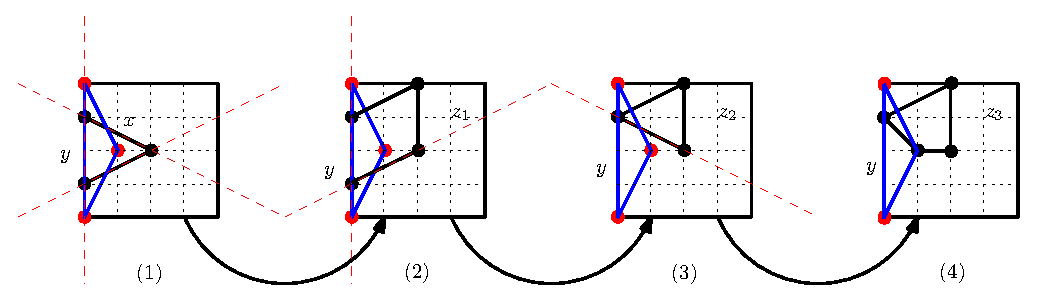
\includegraphics[scale=0.7]{assets/transfo}
      \caption{Ici pour $x$ et $y \in [0,4]^2$, avec $|x \bigtriangleup y| = 6$. On trouve un $z_3 \in \Omega$, tel que $|x \bigtriangleup y| > |z_3 \bigtriangleup y| = 5$, pour lequel on a $\delta(x,z_3) = 3$.}
      \label{fig:transfo}
    \end{center}
  \end{figure}
\end{proof}

% \begin{proposition}\label{prop:prop2}
%   Tout $(d,k)$-polytope peut se réduire à un simplexe de $[0,k]^d$, et de même à partir d'un simplexe de $[0,k]^d$, on peut atteindre $(d,k)$-polytope.
% \end{proposition}
%
% \begin{proof}
%   Deux choses sont à prouver:
%   \begin{enumerate}[i]
%     \item À partir d'un polytope, on peut se réduire à un simplexe.
%
%     Soit $x,y \in \Omega$, avec $|x| = l$ et $|y| = d+1$. On suppose que $y$ n'est pas encore défini mais on sait seulement que sa taille est de $d+1$, on suppose également que $l$ est suffisament grand par rapport à $d+1$. On remarque que $y$ est un simplexe de dimension $d$. Prouver que le polytope $x$ peut se réduire à un simplexe signifie qu'on peut trouver un $r>0$ et un $y$ tel que:
%     \begin{equation}
%       P^r(x,y)>0
%     \end{equation}
%     Considérons maintenant une marche dans $X_t$ tel que $X_0 = x$. Cette marche consiste à choisir à chaque étape la transition qui enlève à $x$ exactement son $i$-ème sommet et s'arrêter quand l'état de la marche est un état de taille $d+1$.
%
%     Soit $z_i \in \Omega$, $z_i$ va correspondre à l'état dans lequel se trouvera la marche après avoir enlevé le $i$-ème sommet de $x$. On a alors la séquence d'états suivante:
%
%     \begin{equation}\label{eq:eq11}
%       \left\{
%       \begin{array}{rl}
%         z_i &= z_{i-1} - \{v_i\} \  \forall i\geq{1}\\
%         z_0 &= x
%       \end{array}
%       \right.
%     \end{equation}
%
%     En déroulant la récurrence en (\ref{eq:eq11}), on a $z_i = x - \{v_1\} - \dots - \{v_i\}$. On remarque que $z_1 = x -\{v_1\}$ si $|x|>d+1$, d'après nos règles de transition cela implique $P(x,z_1)>0$. En répétant à chaque fois cette opération, en procédant de manière itérative sur les $z_i$, on a $P^i(x,z_i)>0$ si $|z_{i-1}|>d+1$. À l'étape $k = l-d-1$ marche atteint $z_k$, avec $|z_k|=d+1$. On choisit alors $r=k=l-d-1$ et $y=z_k$
%
%     \item À partir d'un simplexe, on peut atteindre un polytope.
%
%     On utilise alors un raisonemment analogue en considérant la marche inverse. De plus les règles de transition nous assure que si $P(x,z_1)>0$ alors $P(z_1,x)>0$.
%
%   \end{enumerate}
% \end{proof}

Une fois ces propositions établies, passons à la preuve du théorème \ref{thm1}.

\begin{proof}
  La preuve du théorème \ref{thm1} se fera en trois étapes:

  \begin{enumerate}[i]
    \item \textit{Irréductibilité}

    Rapellons que $X_t$ est irréductible si à partir d'un état on peut atteindre n'importe quel état de $\Omega$ en un temps fini, i.e. on peut trouver un $r_0$ fini tel que pour tout $x_1,x_2 \in \Omega$, $P^r(x_1,x_2)>0 \  \mbox{dès que } r\geq{r_0}$. Soient $x_1,x_2 \in \Omega$. Considérons ensuite deux simplexes $y_1$ et $y_2$ de $\Omega$.

    À completer $\dots$

    \item \textit{Symétrie}

    On rappelle que $X_t$ est symétrique si et seulement si pour tout état $x$ et $y$ de $\Omega$, $P(x,y) = P(y,x)$.

    Soient $x$, $y \in \Omega$, deux états distincts. La relation de transition entre $x$ et $y$ est donnée par nos règles de transition: elle consiste à ajouter ou retirer un unique sommet - voir Figure \ref{fig:fig2}.

    Observons que si il n'existe pas de transition en une étape de $x$ en $y$, $P(x,y)=0$, par conséquent si $P(x,y)=0$ alors $P(y,x)=0$.

    Prouvons ensuite que si $P(x,y)>0$ et $P(y,x)>0$ alors $P(x,y) = P(y,x)$. $P(x,y)>0$ signifie que l'on a une transition de $x$ en $y$ et deux cas peuvent se présenter: soit $y = x - \{v\}$, soit $y = x \cup \{v\}$. Étudions le premier cas où $y = x - \{v\}$. Considérons $v$, un point tiré uniformément sur l'ensemble des points entiers de $[0,k]^d$, la probabilité de tirer $v$ et de l'ajouter à l'enveloppe convexe de $x$ i.e. avoir une trasition de $x$ en $y$ est $P(x,y) = \frac{1}{(k+1)^d}$. De même, pour avoir une transition de $y$ en $x$, on tire $v$ dans $[0,k]^d$ tel que $x = y \cup \{v\}$ avec une probabilité $P(y,x) = \frac{1}{(k+1)^d}$. On a alors

    \begin{equation}
      P(x,y) = P(y,x) = \frac{1}{(k+1)^d}
    \end{equation}

    On prouve l'autre cas par un raisonemment analogue.

    \item \textit{Apériodicité}

    Montrer que $X_t$ est apériodique revient à montrer que tous les états de \om ont tous pour période $1$. On rappelle que la période d'un état $x$ est défini comme étant le $\mathrm{pgcd}(\mathcal{T}(x))$ où $\mathcal{T}(x) = \{t\geq{1} \ : P^t(x,x)>0\}$, c'est l'ensemble des temps $t$ pour lesquels on a $\mathbf{P}\{X_t = x | X_0 = x\}>0$.

    Si $X_t$ est irréductible la propriété \ref{prop1} nous dit que tout les états ont la même période. Par conséquent pour tout $x,y \in \Omega$, $\mathrm{pgcd}(\mathcal{T}(x)) = \mathrm{pgcd}(\mathcal{T}(y))$. Pour prouver que cette période vaut 1, il nous suffit de trouver un $x$ tel que $\mathrm{pgcd}(\mathcal{T}(x)) = 1$.

    Soit $x$ un simplexe de $\Omega$ avec $|x| = d+1$. Par définition de nos règles de transition, après avoir tirer le point $v$ dans $[0,k]^d$, on a la possibilité de boucler sur $x$ pour les cas suivants: soit $v$ est un point intérieur à $x$, soit $v \in x$, soit $v$ est tiré à l'extérieur de $x$ mais $|x \cup \{v\}| \neq |x| + 1$. En termes de probabilités on a: $P(x,x) = \mathbf{P}\{v \  \mbox{un point intérieur à} \ x\} + \mathbf{P}\{v \in x\} + \mathbf{P}\{|x \cup \{v\}| \neq |x| + 1\}$.

    On observe que $\mathbf{P}\{v \in x\} = \frac{1}{(k+1)^d}$ mais puisqu'on a choisi $x$ tel que $|x| = d+1$, on boucle sur $x$ avec probabilité:

    \begin{equation}\label{eq:eq12}
      P(x,x) \geq{\frac{1}{(k+1)^d}} > 0
    \end{equation}

    (\ref{eq:eq12}) nous dit qu'avec une probabilité non nulle on peut revenir en $x$ en partant de $x$ en une étape. Dès lors, $\mathcal{T}(x)$ est de la forme $\mathcal{T}(x) = \{1, \dots\}$. Donc $\mathrm{pgcd}(\mathcal{T}(x)) = 1$.

  \end{enumerate}
\end{proof}

\begin{corollary}\label{coro1}
  Le générateur $\Gamma(d,k)$ décrit par l'algorithme \ref{algo1} est un générateur aléatoire uniforme de $(d,k)$-polytopes.
\end{corollary}

\begin{proof}
  La construction de $\Gamma(d,k)$ se base sur le modèle d'une marche sur $X_t$. La preuve est immédiate et découle du théorème \ref{thm1}.
\end{proof}



\clearpage
\bibliographystyle{plain}
\bibliography{biblio.bib}

\end{document}
